In Figure \ref{fig:flow1} the fluid flow velocity is plotted. Parabolic behaviour is observed closer to the edges as is expected. Now let's see what happens to the flow if objects are placed in the flow.

\begin{figure}[ht!]
\centering
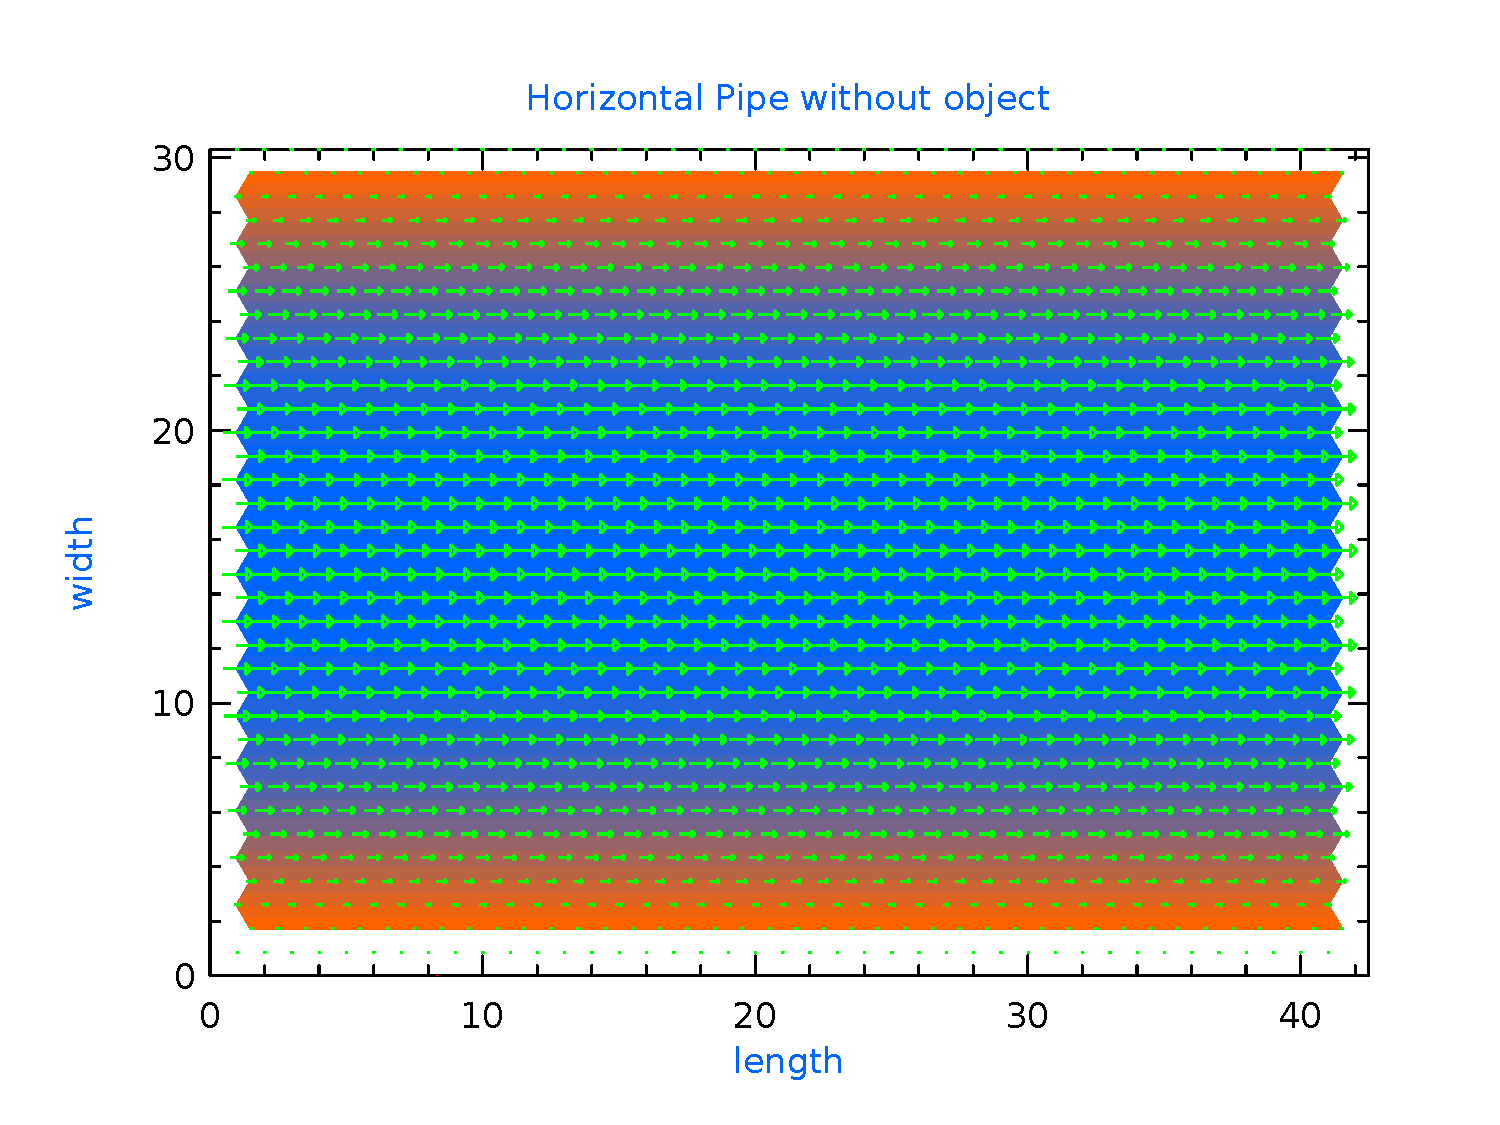
\includegraphics[width=.7\textwidth]{plots/flow.pdf}
\caption{Horizontal flow in a pipe. The arrows give an indication of the velocity at that point, the color indicates the horizontal velocity. Low velocities correspond to orange, high velocities to blue. }
\label{fig:flow1}
\end{figure}



In Figure \ref{fig:flow2} snapshots are seen depecting various (non) moving objects in the horizontal pipe flow. The flow neatly goes around the objects. It should be noted that the objects are moving, except in Figure 2a.

\begin{figure}[ht!] \flushleft
  \subfloat[Non-moving rectangle placed in the laminar flow.]{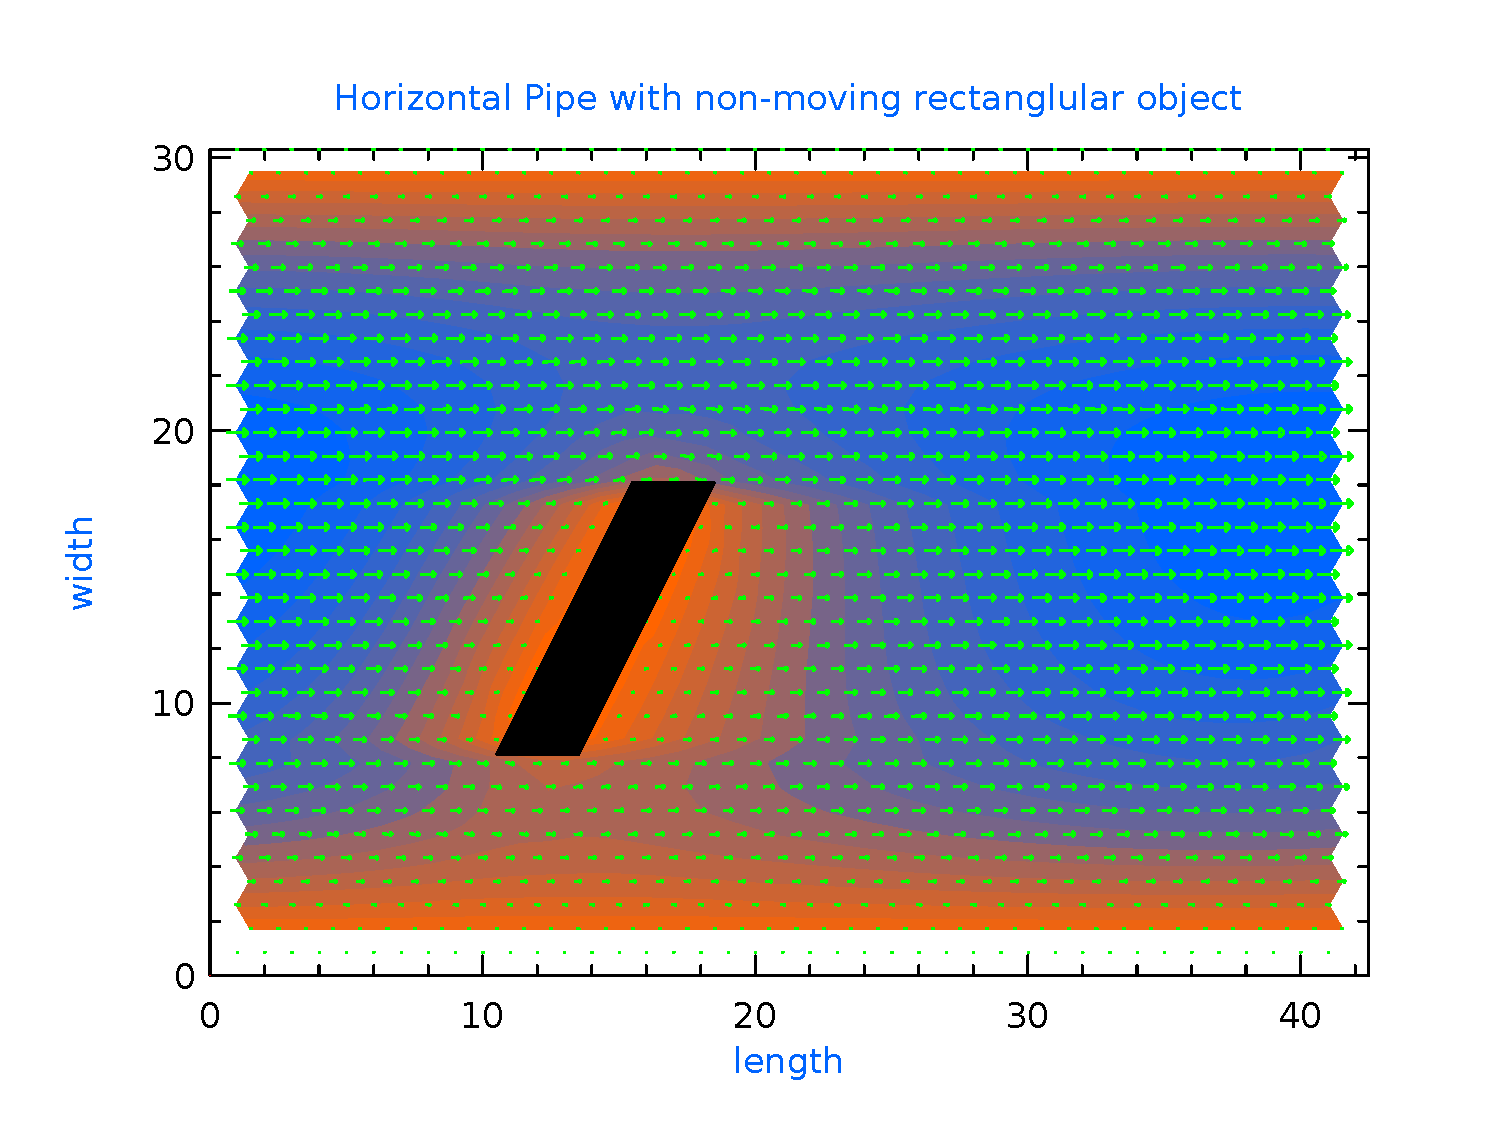
\includegraphics[width=.47\textwidth]{plots/rectangle.pdf}\label{fig:rectangle}} 
  \subfloat[Moving square placed in the laminar flow. It is placed near the middle of the flow so it hardly rotates.]{\label{fig:square}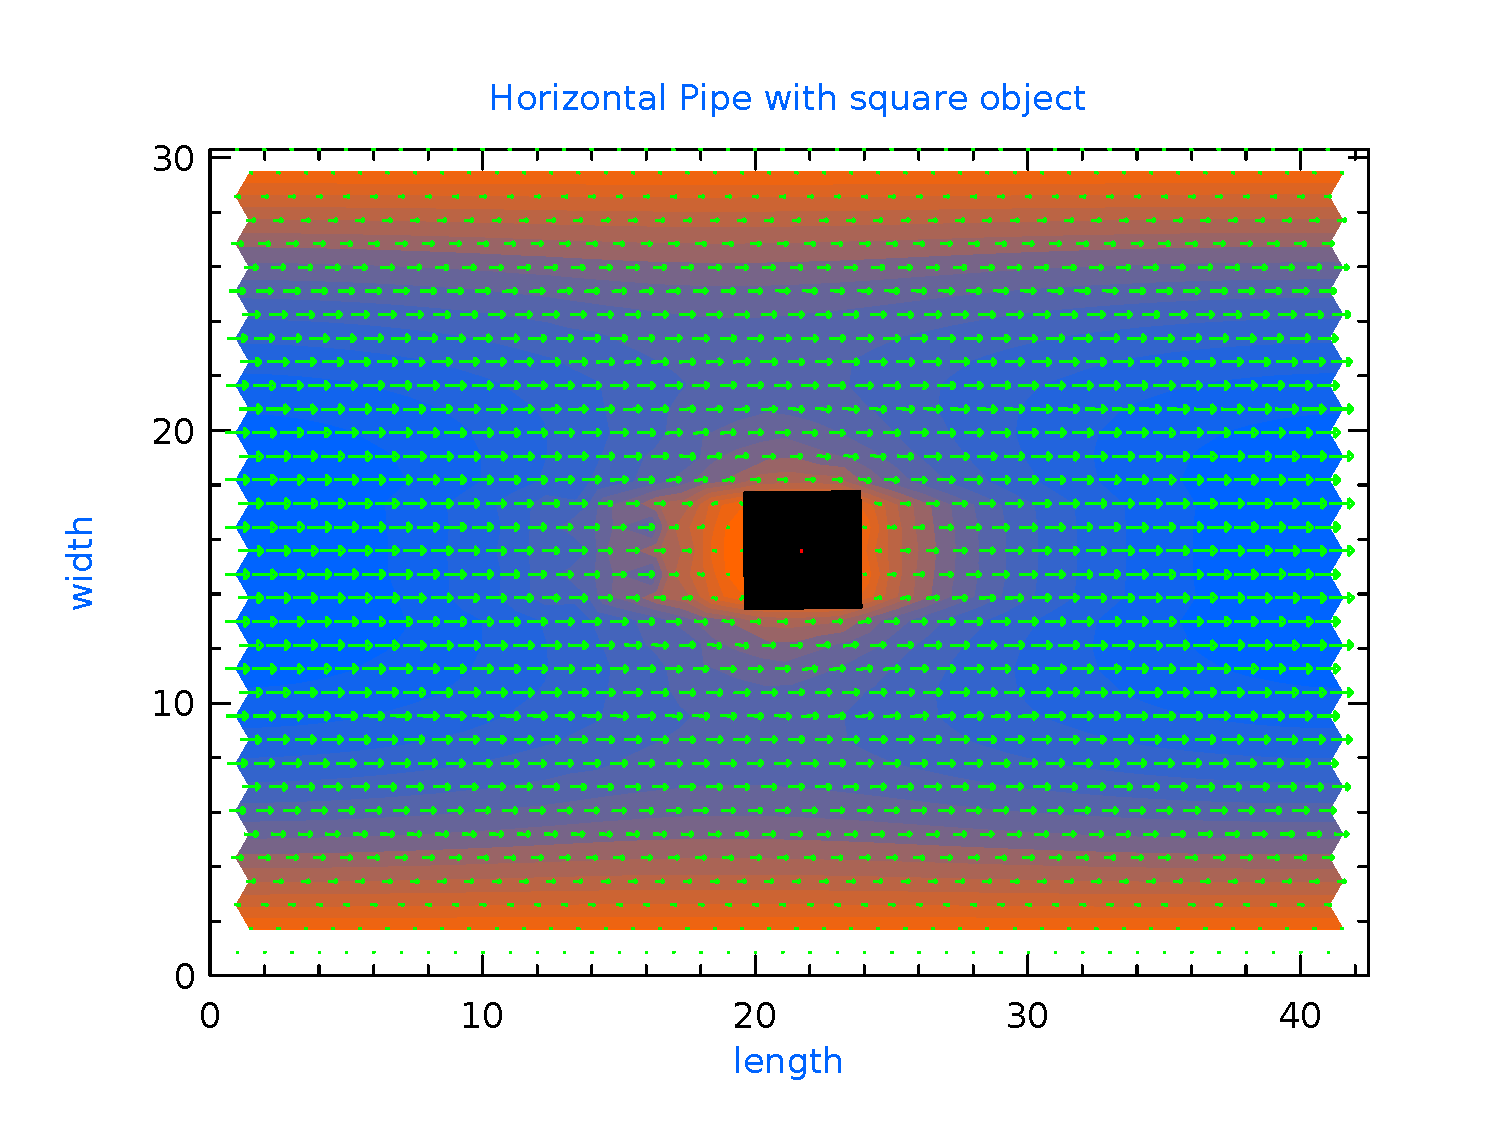
\includegraphics[width=.47\textwidth]{plots/square.pdf} }    \\
  \subfloat[Moving square placed in the laminar flow. It is placed near the edge of the flow so it rotates.]{\label{fig:rotating_square}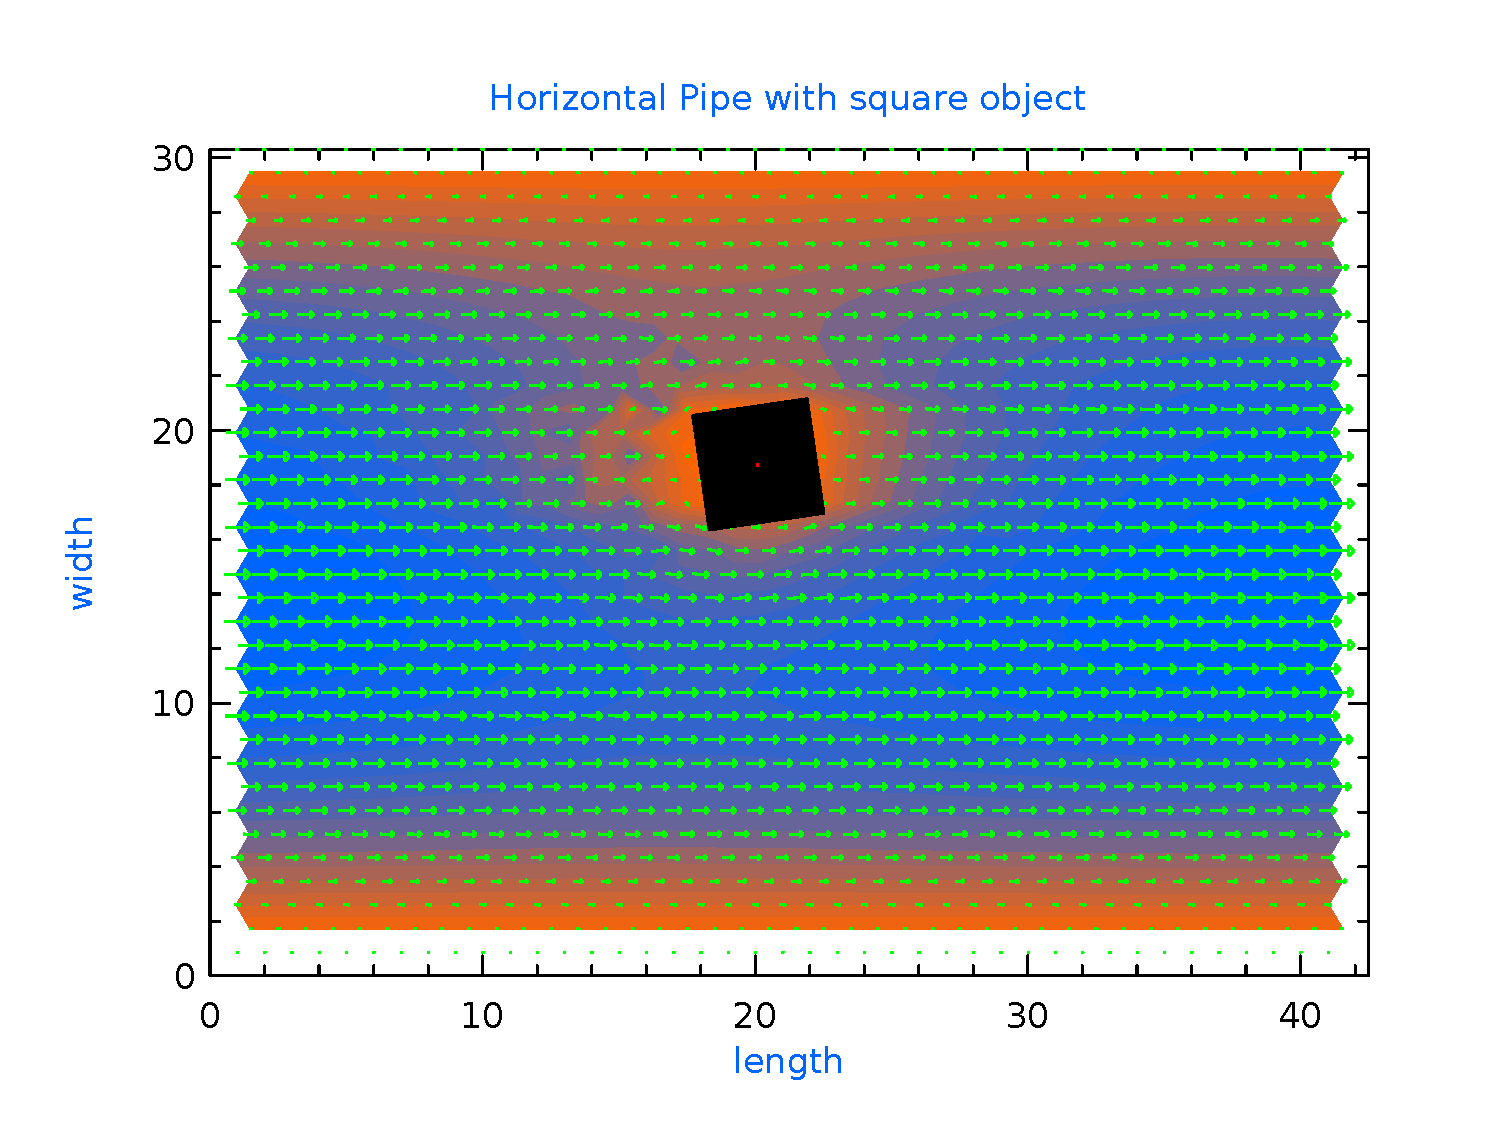
\includegraphics[width=.47\textwidth]{plots/rotating_square.pdf}} 
  \subfloat[Moving sphere placed in the laminar flow.]{\label{fig:sphere}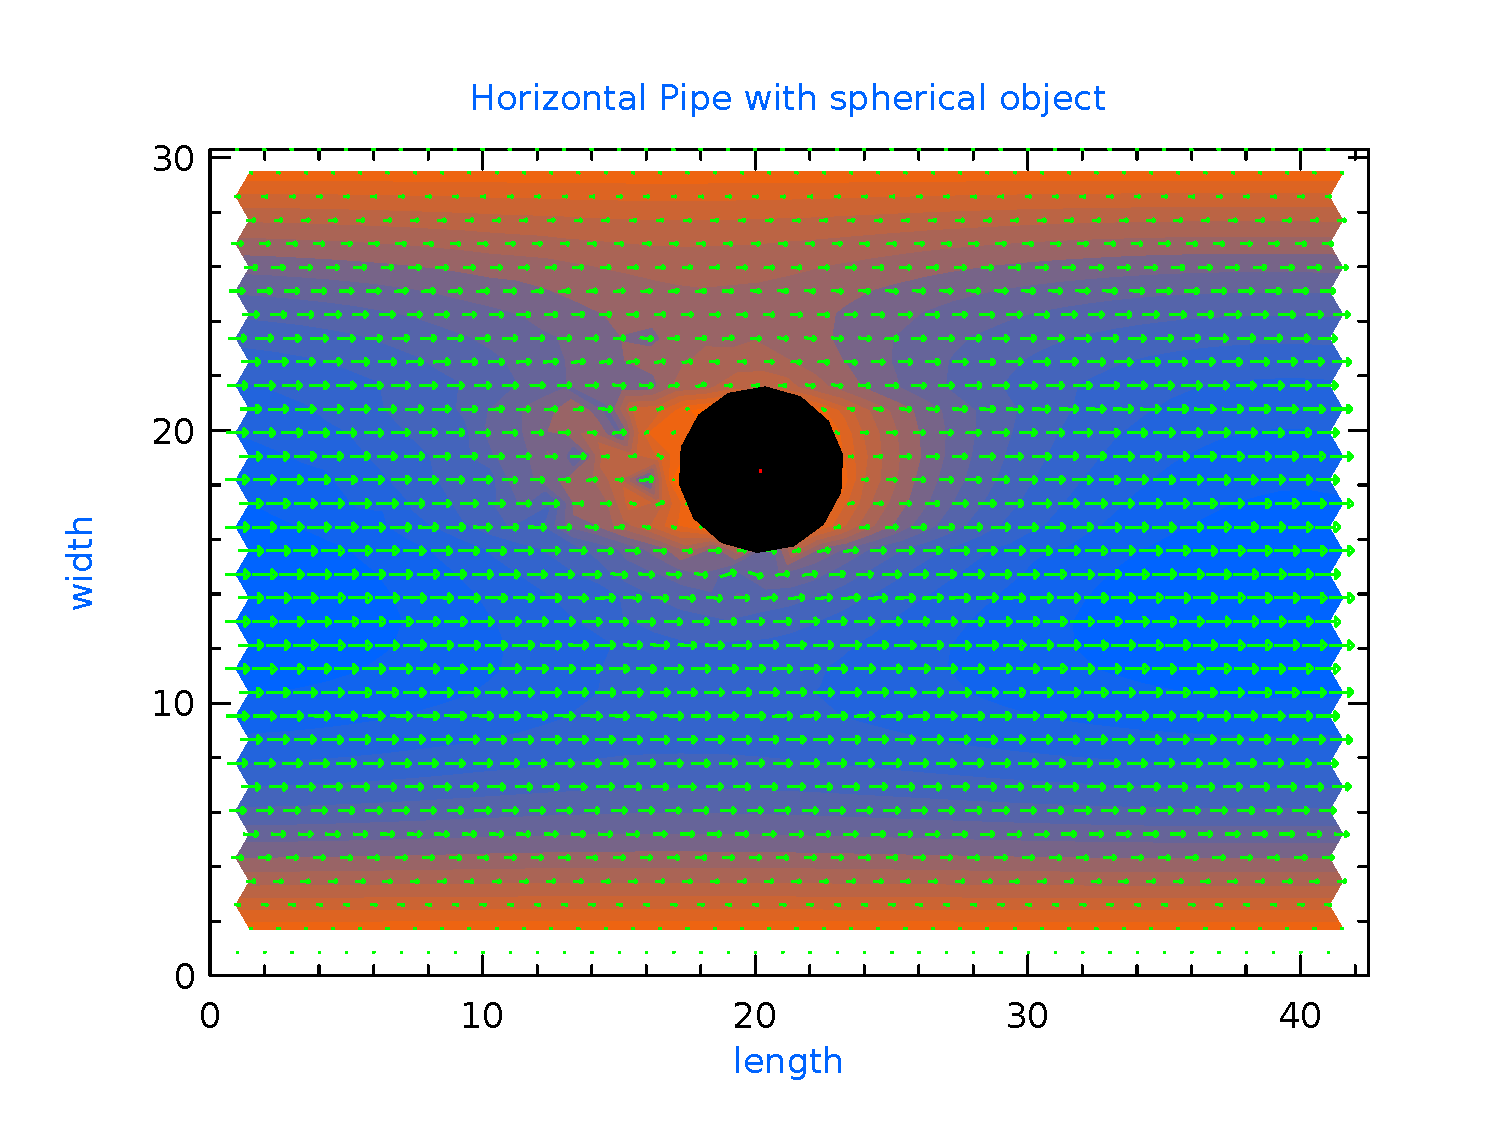
\includegraphics[width=.47\textwidth]{plots/sphere.pdf} }  \\
  \subfloat[Moving triangle placed in the laminar flow.]{\label{fig:triangle}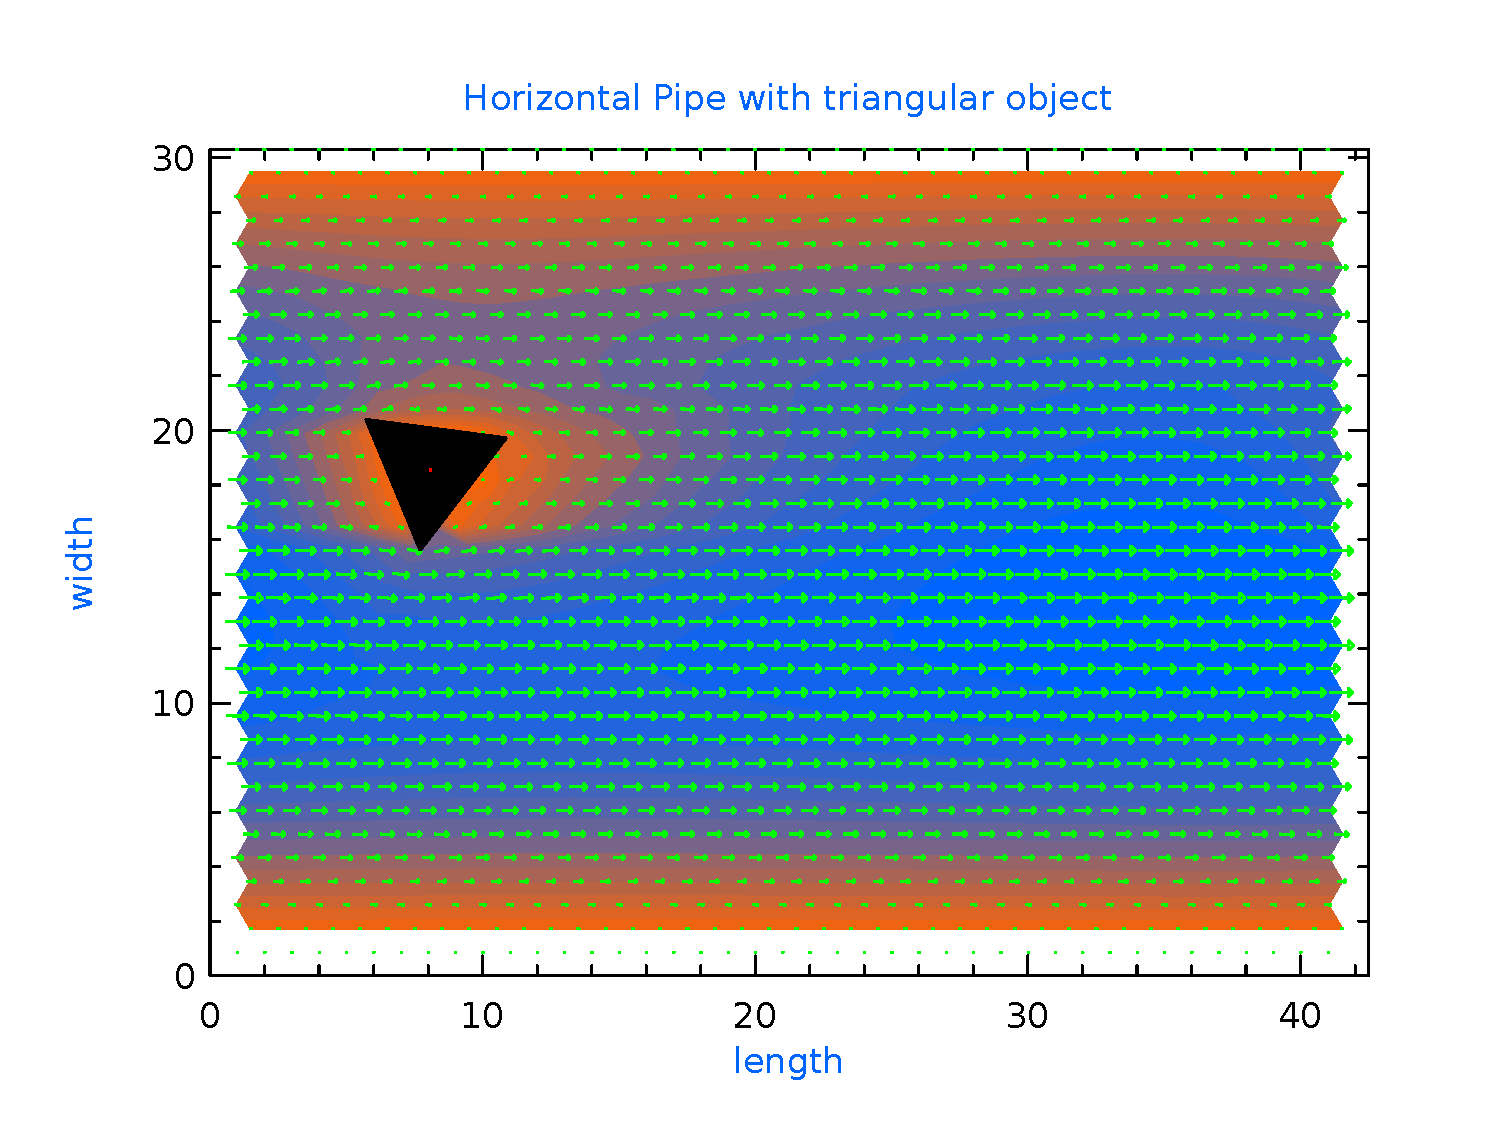
\includegraphics[width=.47\textwidth]{plots/triangle.pdf}} 
  \subfloat[Moving hexagon placed in the laminar flow. The mass distribution is non uniform which influences its rotation.]{\label{fig:hexagon}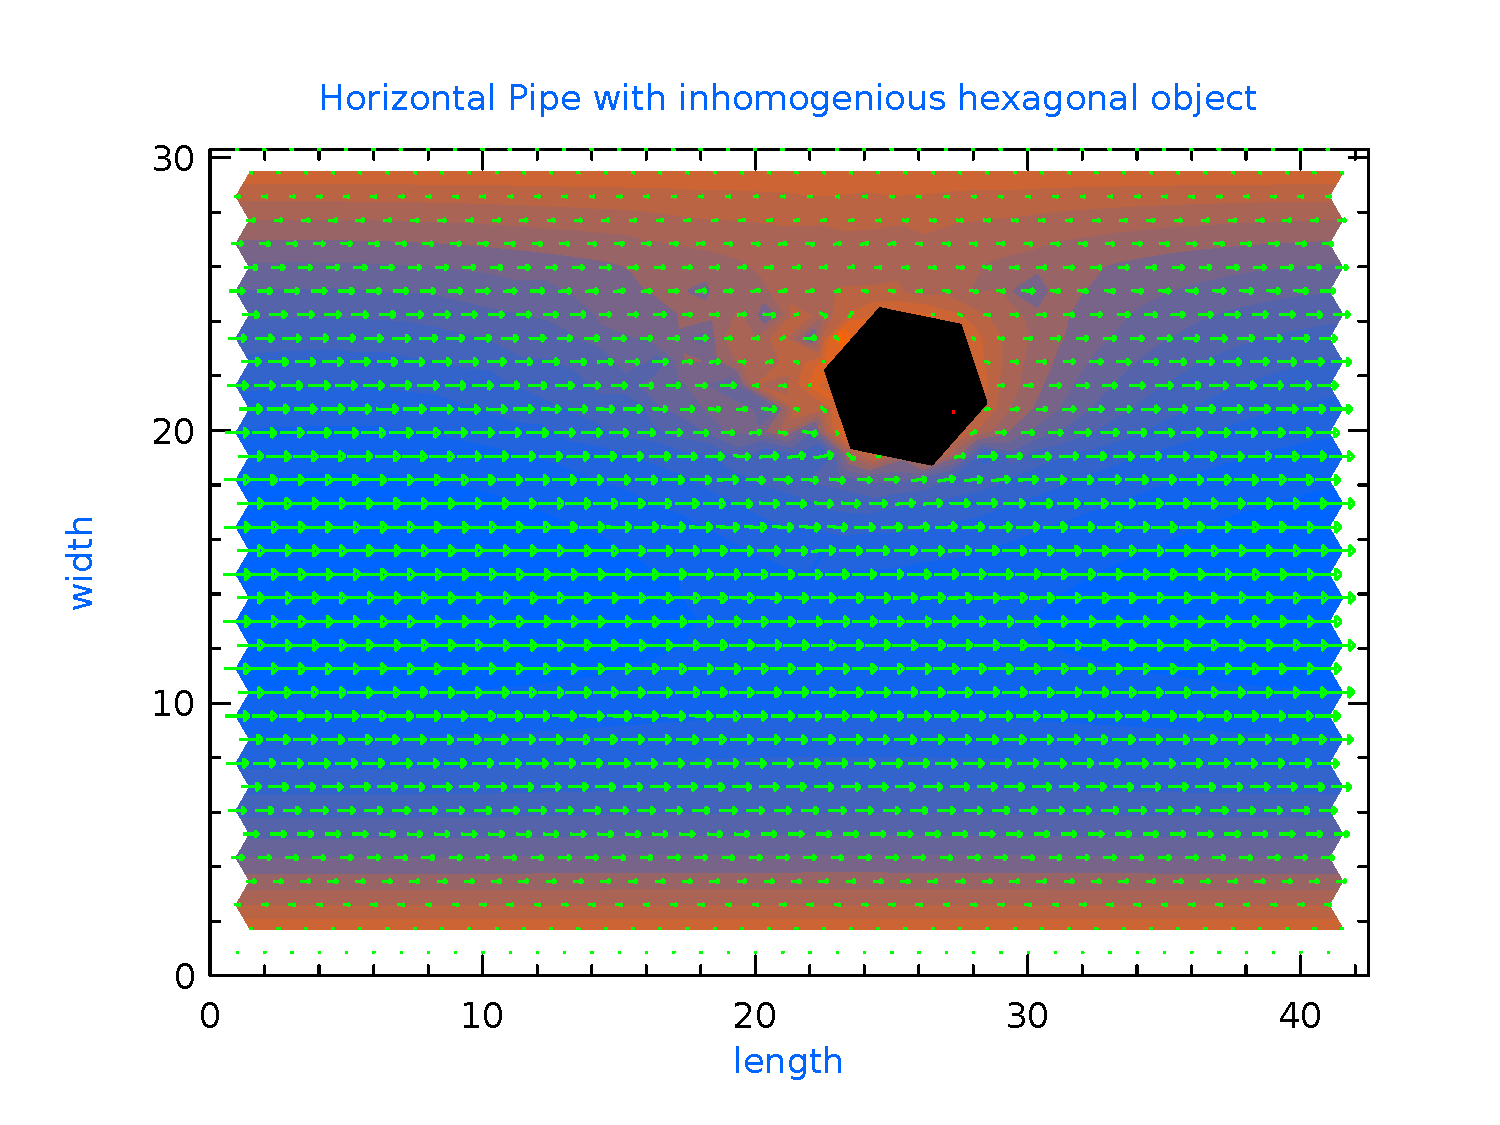
\includegraphics[width=.47\textwidth]{plots/hexagon.pdf} }    
       
 \caption{Objects placed in laminar flow. The arrows give an indication of the velocity at that point, the color indicates the horizontal velocity. Low velocities correspond to orange, high velocities to blue. The red dot is the position of the centre of mass of the object. }
\label{fig:flow2}

\end{figure}
